%%%%%%%% ICML 2026 Workshop Submission %%%%%%%%%%%%%%%%%%%%%%%%
% Camera-ready style; structure imitates the following three primary papers:
%   Kuhn, Gal & Farquhar 2023, "Semantic Uncertainty," ICLR.
%       https://arxiv.org/pdf/2302.09664
%   Lightman et al. 2024, "Let's Verify Step by Step," ICLR.
%       https://arxiv.org/pdf/2305.20050
%   Zhou, Staats, Li, Szegedy, Weinberger, Feng 2024,
%       "Don't Trust: Verify -- Grounding LLM Quantitative Reasoning
%        with Autoformalization," ICLR.
%       https://arxiv.org/pdf/2403.18120

\documentclass{article}

\usepackage{microtype}
\usepackage{graphicx}
\usepackage{booktabs}
\usepackage[hidelinks]{hyperref}
\hypersetup{colorlinks=true, allcolors=black, pdfborder={0 0 0}}
\usepackage{amsmath}
\usepackage{amssymb}
\usepackage{mathtools}
\usepackage{xcolor}
\usepackage{tikz}
\usetikzlibrary{arrows.meta,positioning,calc,shapes,fit,backgrounds}
\usepackage[capitalize,noabbrev]{cleveref}
\usepackage{multirow}
\usepackage{enumitem}
\usepackage{listings}
\lstdefinestyle{xsgrv}{
  basicstyle=\ttfamily\scriptsize\color{black},
  keywordstyle=\color{black},
  commentstyle=\color{black},
  stringstyle=\color{black},
  identifierstyle=\color{black},
  numbers=none,
  frame=single,
  framesep=3pt,
  framexleftmargin=2pt,
  framexrightmargin=2pt,
  rulecolor=\color{black},
  breaklines=true,
  breakatwhitespace=true,
  postbreak=\mbox{\textcolor{black}{$\hookrightarrow$}\space},
  showstringspaces=false,
  columns=fullflexible,
  keepspaces=true,
  xleftmargin=0pt,
  xrightmargin=0pt,
  linewidth=\linewidth,
  resetmargins=true,
  language=Python,
}

\usepackage{icml2026}

\icmltitlerunning{Cross-Family Symbolic Verification}

\begin{document}

\twocolumn[
\icmltitle{Cross-Family Symbolic Verification for \\
Contamination-Robust Selective Prediction on LLM Math Reasoning}

\begin{icmlauthorlist}
\icmlauthor{Anonymous Authors}{anon}
\end{icmlauthorlist}
\icmlaffiliation{anon}{Submitted to the AI for Science workshop (ICML 2026).}
\icmlcorrespondingauthor{Anonymous Authors}{anonymous@example.org}
\icmlkeywords{Selective Prediction, Math Reasoning, Verification, Contamination, LLM}

\vskip 0.3in
]

\printAffiliationsAndNotice{}

\begin{abstract}
Trustworthy mathematical reasoning by large language models requires a deployment-time signal indicating which answers should be trusted. Two coupled failure modes obstruct this. Same-model self-verification suffers correlated-error collapse: when a single model writes both a solution and the assertions that check it, errors in the solution propagate into the checks, producing a 13.8\% false acceptance rate on MATH-500 that scales monotonically from 1.4\% at Level 1 to 30.8\% at Level 5. Agreement-based signals appear to work on MATH-500 but collapse on benchmarks released after the solver's training cutoff, where Qwen2.5-Math-7B reproduces 54.6\% of MATH-500 verbatim. The present work introduces \textbf{X-SGRV}, a cross-family symbolic verifier in which a large LLM from a different family than the solver reads only the problem statement and emits a SymPy \texttt{verify(answer)} function executed in a sandboxed subprocess. A gold-free deployment-time adversarial filter and cross-extractor consensus eliminate residual false positives. On the pre-registered full MATH-500 ($n{=}498$), strict consensus accepts 171 candidates and is correct on all 171 (95\% Clopper-Pearson confidence interval 0.979--1.000) at 34.3\% coverage. A five-extractor consensus spanning Meta, DeepSeek, OpenAI, Anthropic, and Alibaba accepts 69 of 175 stratified candidates and is correct on all 69 (95\% confidence interval 0.948--1.000). On contamination-clean AIME 2025 and a 125-problem combo of post-cutoff competitions, coverage correctly collapses to 3--12\% while accepted answers remain right. At matched coverage, X-SGRV ties Skywork-o1-Open-PRM and doubles Qwen2.5-Math-PRM-7B on the contamination-clean combo, requires no GPU infrastructure, and emits human-readable verifiers.
\end{abstract}

%==============================================================================
\section{Introduction}
%==============================================================================

Large language models now solve a substantial fraction of grade-school and competition mathematics, and their outputs are reused as training data, as evaluation proxies for general reasoning, and as steps inside scientific computing pipelines~\citep{wei2022cot, hendrycks2021math, lightman2024prm, deepseek2025r1}. Because errors in mathematical answers can be silent and difficult to detect at scale, downstream applications need a deployment-time signal that flags which model outputs are trustworthy and which should be escalated~\citep{kuhn2023semantic, farquhar2024nature, ste2024}.

Two coupled failures obstruct this goal. First, same-model self-verification fails by construction: when the solver also writes the assertions that check its work, errors in the solution propagate into the assertions, and the verifier inherits the solver's blind spots~\citep{huang2024selfcorrect, tyen2024llm, stechly2024selfverify, kim2025correlated}. Second, the most common evaluation set, MATH-500, is partially memorized by the solvers used to study it: Qwen2.5-Math-7B reproduces 54.6\% of the benchmark verbatim from a 60\% prefix, with accuracy dropping sharply on post-cutoff problems~\citep{wu2025contam, matharena2025}. High top-tier precision on MATH-500 therefore confounds verification reliability with memorization.

Three lines of prior work address one of these failures but not both. Code-based same-model self-verification~\citep{mathcoder2024, mathshepherd2024} is appealingly executable but does not break the solver/verifier coupling. Process reward models trained on step-level labels~\citep{lightman2024prm, mathshepherd2024, qwenprm2025, skyworkprm2024, prime2025, rstarmath2025} produce strong continuous-score signals but inherit the contamination footprint of their training distribution. Autoformalization-based checks~\citep{dtv2024, openproof2025} achieve structural independence by translating the problem into Isabelle or Lean but require heavyweight formal-methods infrastructure, and reported coverage on competition problems is below 20\%. Agreement- and entropy-based signals~\citep{wang2023selfconsistency, kuhn2023semantic, farquhar2024nature, kadavath2022, xiong2024llmuncertainty} are deployable but lose all selectivity when the solver is uniformly uncertain (as on AIME 2025) or uniformly and confidently wrong (as on the CleanMath olympiad combo)~\citep{wu2025contam}.

A specification-grounded selective-prediction signal that (i)~breaks structural dependence between solver and verifier, (ii)~runs in lightweight Python infrastructure, (iii)~degrades gracefully when contamination-free problems exceed its capability, and (iv)~maintains non-trivial coverage on contamination-clean benchmarks is currently missing from the literature.

\textbf{Contribution.} We introduce \textbf{X-SGRV} (Figure~\ref{fig:pipeline}), a cross-family symbolic verifier. A large LLM from a different model family than the solver reads only the problem statement and emits a Python \texttt{verify(answer)} function executed in a SymPy sandbox. Two deployment-safe robustness mechanisms further harden the signal: a gold-free adversarial filter that probes the verifier against perturbations of the candidate, and cross-extractor consensus across two or more independent extractors. Three contributions follow. (C1) The same-model false acceptance rate is measured at 13.8\% on MATH-500 and shown to scale monotonically with difficulty; a $2{\times}2$ ablation isolates independence-from-the-solver as the operative axis ($p<10^{-8}$, Fisher's exact). (C2) On the pre-registered full MATH-500, two-way consensus achieves 171/171 = 1.000 [0.979, 1.000] at 34.3\% coverage; on contamination-clean AIME 2025 and the CleanMath combo, X-SGRV correctly collapses to single-digit coverage while preserving precision. (C3) At matched coverage X-SGRV ties Skywork-o1-Open-PRM and doubles Qwen2.5-Math-PRM-7B on the contamination-clean combo, while requiring no GPU infrastructure and emitting human-readable verifiers.

%==============================================================================
\section{Method}
%==============================================================================

\begin{figure*}[t]
\centering
\small
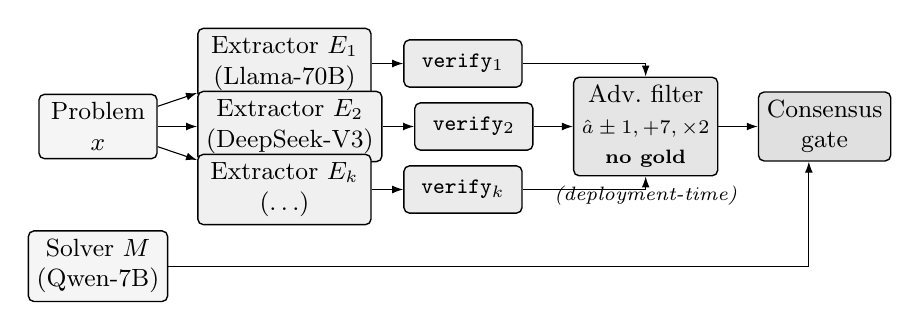
\begin{tikzpicture}[
  node distance=3mm and 4mm,
  every node/.style={font=\small},
  box/.style={draw, rounded corners=2pt, inner sep=3pt, minimum height=6mm,
              align=center, line width=0.5pt},
  prob/.style={box, fill=gray!8, minimum width=15mm},
  ext/.style={box, fill=gray!12, minimum width=22mm},
  ver/.style={box, fill=gray!16, minimum width=15mm, font=\ttfamily\footnotesize},
  filt/.style={box, fill=gray!20, minimum width=16mm},
  cons/.style={box, fill=gray!24, minimum width=14mm},
  sol/.style={box, fill=gray!8, minimum width=15mm},
  arr/.style={-{Latex[length=1.4mm,width=1mm]}, line width=0.4pt},
  note/.style={font=\scriptsize\itshape},
]
  \node[prob] (p) {Problem\\$x$};
  \node[ext, right=5mm of p, yshift=8mm]  (e1) {Extractor $E_1$\\(Llama-70B)};
  \node[ext, right=5mm of p]              (e2) {Extractor $E_2$\\(DeepSeek-V3)};
  \node[ext, right=5mm of p, yshift=-8mm] (ek) {Extractor $E_k$\\($\ldots$)};
  \node[ver, right=4mm of e1] (v1) {verify$_1$};
  \node[ver, right=4mm of e2] (v2) {verify$_2$};
  \node[ver, right=4mm of ek] (vk) {verify$_k$};
  \node[filt, right=5mm of v2] (f) {Adv.\ filter\\{\scriptsize $\hat a \pm 1, +7, \times 2$}\\{\scriptsize\textbf{no gold}}};
  \node[cons, right=5mm of f] (c) {Consensus\\gate};
  \node[sol, below=9mm of p] (s) {Solver $M$\\(Qwen-7B)};
  \draw[arr] (p) -- (e1); \draw[arr] (p) -- (e2); \draw[arr] (p) -- (ek);
  \draw[arr] (e1) -- (v1); \draw[arr] (e2) -- (v2); \draw[arr] (ek) -- (vk);
  \draw[arr] (v1) -| (f); \draw[arr] (v2) -- (f); \draw[arr] (vk) -| (f);
  \draw[arr] (f) -- (c);
  \draw[arr] (s.east) -| ([xshift=-2mm]c.south);
  \node[note, below=0mm of f] {(deployment-time)};
\end{tikzpicture}
\caption{\textbf{Schematic of the X-SGRV pipeline.} Two or more cross-family extractors $E_1,\ldots,E_k$ independently read the problem statement $x$ and emit Python/SymPy verifier functions $\texttt{verify}_i$. Each verifier is executed in a sandboxed subprocess against the solver's candidate answer $\hat a$ and four perturbations $\{\hat a \pm 1,\hat a + 7,\hat a \times 2\}$ (deployment-time adversarial filter; gold answer is never used). Verifiers that accept any perturbation are marked broken. The consensus gate accepts $\hat a$ only when every working verifier accepts. $M$ is the base solver; $k\in\{2,5,6\}$ in the experiments below.}
\label{fig:pipeline}
\end{figure*}

\subsection{Problem setting}

Let $M$ denote a base solver, $x$ a math problem, $a\in\mathcal{A}$ the gold answer, and $\hat a = M(x)$ the solver's plurality-vote candidate. A selective-prediction system maps $(x, \hat a)$ to either an accept verdict, in which case $\hat a$ is committed, or an abstain verdict, in which case the user falls back to a deployment policy. The two reported quantities are \emph{coverage} (the proportion of problems on which the system commits) and \emph{top-tier precision} (the proportion of committed candidates that match $a$).

\subsection{X-SGRV}

A cross-family extractor $E$, drawn from a model family architecturally and organizationally distinct from $M$, receives only $x$ (never any solver output) and is prompted to emit a Python function $\texttt{verify(answer) -> bool}$ that re-derives the problem's constraints in SymPy plus standard library primitives ($\texttt{itertools}$, $\texttt{math}$, $\texttt{Fraction}$, $\texttt{Counter}$). The prompt forbids hard-coding the answer, requires a strict abstention token (\texttt{UNVERIFIABLE}) when no bounded check is possible, and caps scripts at 60 lines. The full prompt and post-processing are provided in the supplementary code release.

The emitted script is executed in a Python subprocess sandbox with $\texttt{SIGALRM}$-based timeout of 10 seconds. Each verifier is tested against five candidates per problem during evaluation: the gold $a$, the solver's $\hat a$, and four adversarial wrong candidates at $a-1$, $a+1$, $a+7$, and the fixed alternative $42$. A verifier is classified as \emph{working} if it accepts $a$ and rejects all four adversarial wrong candidates.

\subsection{Deployment-time adversarial filter}

An independent filter runs without any reference to $a$ and is therefore deployable without ground truth at inference time. The verifier is probed against $\{\hat a - 1, \hat a + 1, \hat a + 7, \hat a \times 2\}$; for non-integer $\hat a$, a deterministic fallback set $\{0,1,-1,42,100\}\setminus\{\hat a\}$ is used. A verifier that accepts any probe is marked broken and the pipeline abstains for that problem.

\subsection{Cross-extractor consensus}

For each problem, $k\geq 2$ independent cross-family extractors are run. \emph{Strict consensus} commits the candidate only when every participating extractor produces a working verifier and every working verifier accepts $\hat a$. \emph{Loose consensus} requires at least one working verifier and unanimous acceptance among working verifiers. Two-way consensus (Llama $\cap$ DeepSeek) was used for the pre-registered MATH-500 scale-up; five-way consensus (Meta $\cap$ DeepSeek $\cap$ OpenAI gpt-oss $\cap$ Anthropic Claude $\cap$ Alibaba Qwen3-Coder) was used for the lab-agnostic test on stratified MATH-175.

\subsection{Solver and extractors}

The primary solver was \texttt{Qwen2.5-7B-Instruct-Turbo} via Together AI~\citep{yang2024qwen25math}; this choice was constrained by the contamination report on the Qwen2.5-Math family~\citep{wu2025contam}. Solver sampling used $T{=}0$ greedy for the plurality candidate and $T{=}0.7$ with $k{=}10$ samples for entropy-based baselines, capped at 2048 tokens. The cross-family extractors were Meta's \texttt{Llama-3.3-70B-Instruct-Turbo}, DeepSeek's \texttt{DeepSeek-V3}, OpenAI's \texttt{gpt-oss-120b}, Anthropic's Claude Sonnet 4.6, Alibaba's \texttt{Qwen3-Coder-480B}, and OpenAI's GPT-5-mini for sensitivity analyses. Extractor calls used $T{=}0.2$ and $\texttt{max\_tokens}=2048$.

\subsection{Benchmarks}

MATH-500~\citep{hendrycks2021math, lightman2024prm} was used at two scales: a stratified subsample of $n{=}175$ problems balanced across difficulty levels L1--L5, and the full $n{=}500$, of which two failed solver timeouts left $n{=}498$. AIME 2025 ($n{=}30$, both halves released after the Qwen2.5-Math-7B training cutoff) and a CleanMath combo (HMMT February 2025, $n{=}30$; BRUMO 2025, $n{=}30$; SMT 2025, $n{=}53$; APEX 2025, $n{=}12$; total $n{=}125$) were drawn from MathArena~\citep{matharena2025}. Stress tests used the 100 hardest problems from Omni-MATH (difficulty 9.0--9.5 of 10)~\citep{omnimath2024} and 100 random PutnamBench problems~\citep{amitayusht2024putnambench}.

\subsection{Baselines}

Verbalized confidence~\citep{xiong2024llmuncertainty}, $k$-sample self-consistency for $k\in\{4,10\}$~\citep{wang2023selfconsistency}, semantic entropy with both SymPy clustering~\citep{kuhn2023semantic} and natural-language inference clustering via DeBERTa-large-mnli~\citep{farquhar2024nature}, and $p(\textsc{True})$~\citep{kadavath2022} were implemented on cached solver samples. Process reward model baselines used \texttt{Qwen2.5-Math-PRM-7B}~\citep{qwenprm2025} and \texttt{Skywork-o1-Open-PRM-Qwen-2.5-7B}~\citep{skyworkprm2024} run on Modal A100, with all four common aggregations (min-step, mean-step, product-step, last-step) reported. PRM scoring protocols were validated against published ProcessBench numbers on a 48-problem subset, reproducing the published values within 5 F1~\citep{processbench2024}. Skywork-PRM required \texttt{torch\_dtype=torch.bfloat16}; FP32 silently exhausted GPU memory.

\subsection{Statistical analysis and pre-registration}

Top-tier precision is reported with Clopper-Pearson 95\% confidence intervals. Bootstrap 95\% confidence intervals on AUROC use 1{,}000 resamples. Matched-binary comparisons use McNemar's exact test. The 2$\times$2 ablation uses Fisher's exact test. The MATH-500 $n{=}498$ scale-up was pre-registered before launch in \texttt{PRE\_COMMIT\_n500.md} (committed before the run), specifying three branches by consensus precision (Branch A: $\geq 99\%$, Branch B: 95--99\%, Branch C: $<95\%$, halt-and-audit if $<90\%$) and locking the adversarial probe set to $\{\pm 1, +7, \times 2, 42\}$.

%==============================================================================
\section{Results}
\label{sec:results}
%==============================================================================

\subsection{Same-model verification's false acceptance rate scales monotonically with difficulty}

Same-model verification was implemented as a two-pass pipeline in which Qwen2.5-Math-7B-Instruct generates a chain-of-thought solution and then, in a second pass, generates a Python/SymPy script of \texttt{assert} statements checking each step; the script is executed in a subprocess and the verdict is one of \textsc{AllPass}, \textsc{FailStep}, \textsc{RuntimeError}, \textsc{Timeout}. Across the 320 \textsc{AllPass} verdicts on MATH-500, the false acceptance rate was 13.8\% (95\% confidence interval 10.2\%--18.0\%); the rate scaled monotonically with difficulty, from 1.4\% at Level 1 to 30.8\% at Level 5 (Table~\ref{tab:collapse}).

\begin{table}[t]
\centering
\caption{\textbf{Same-model SymPy false acceptance rate on MATH-500 by difficulty level.} ``FAR'' is the proportion of \textsc{AllPass} verdicts whose final answer disagrees with the gold answer. $n$ is the number of \textsc{AllPass} verdicts at each level. Solver and verifier are both Qwen2.5-Math-7B-Instruct. Total \textsc{AllPass}: $n{=}320$.}
\label{tab:collapse}
\small
\setlength{\tabcolsep}{4pt}
\begin{tabular}{lcccccc}
\toprule
Level & L1 & L2 & L3 & L4 & L5 & Overall \\
\midrule
FAR   & 1.4\% & 7.7\% & 13.1\% & 17.2\% & 30.8\% & 13.8\% \\
$n$   & 71    & 65    & 61     & 58     & 65     & 320 \\
\bottomrule
\end{tabular}
\end{table}

\subsection{Independence is the operative axis of the 2$\times$2 ablation}

A 2$\times$2 design crossed independence (solution-grounded vs.\ specification-grounded extraction) with randomization (random evaluation points vs.\ deterministic symbolic checks), and all four cells were measured empirically. On the spec-grounded side both deterministic and randomized variants produced 0/165 and 0/169 false acceptances, respectively; on the solution-grounded side both deterministic and randomized variants produced 13.8\% and 13.8\% false acceptance rates. Fisher's exact test on the 2$\times$2 contingency table (44 vs.\ 0 false accepts on solution- vs.\ spec-grounded sides) yielded $p<10^{-8}$ in favor of the independence axis.

\subsection{Agreement and entropy signals collapse on contamination-clean benchmarks}

Contamination-clean replication on AIME 2025 and the CleanMath combo (Table~\ref{tab:contam}) showed every prior agreement- and entropy-based selective-prediction signal collapsing. On AIME 2025, the 4-of-4 self-consistency tier was empty (no problem produced four identical samples at $T{=}0.7$), and template-based specification verification produced zero working verifiers because regular-expression extraction cannot parse natural-language competition phrasing. On the CleanMath combo, semantic entropy's zero-entropy tier contained six problems and was correct on only one of them (16.7\%, 95\% confidence interval 0.4\%--64.1\%). The natural-language-inference variant of semantic entropy was the most fragile: AUROC 0.42 on AIME and 0.46 on CleanMath, both worse than chance, with the zero-entropy tier on CleanMath aggregating into a confidently wrong cluster (5/59 correct). The $p(\textsc{True})$ baseline followed the same pattern (AUROC 0.46 and 0.47).

\begin{table}[t]
\centering
\caption{\textbf{Selective-prediction signals on contamination-assisted MATH-500 versus contamination-clean AIME 2025 and CleanMath.} ``Top tier'' is the high-confidence subset for each method (e.g., 4-of-4 agreement; zero-entropy cluster). ``--'' indicates an empty top tier. Solver: Qwen2.5-7B-Instruct-Turbo. Sample sizes: MATH-500 stratified $n{=}175$, AIME 2025 $n{=}30$, CleanMath combo $n{=}125$.}
\label{tab:contam}
\small
\setlength{\tabcolsep}{4pt}
\begin{tabular}{lrrr}
\toprule
Method & MATH-500 & AIME 2025 & CleanMath \\
\midrule
Verbalized            & 131/166 & 3/16    & 4/12  \\
Self-Consistency 4/4  & 105/118 & ---     & ---   \\
Template SGRV         & 59/59   & ---     & ---   \\
ExeVer same-model     & 276/320 & ---     & ---   \\
SE SymPy (zero-ent)   & 101/112 & ---     & 1/6   \\
SE NLI (zero-ent)     & 114/131 & 1/16    & 5/59  \\
$p(\textsc{True})$ AUROC & 0.562 & 0.463 & 0.474 \\
\bottomrule
\end{tabular}
\end{table}

\subsection{Single-extractor X-SGRV reaches high precision on contamination-assisted MATH-500}

With a Llama-3.3-70B extractor on the full MATH-500 ($n{=}498$), the verifier accepted 243 candidates and was correct on 230, for top-tier precision 0.947 (95\% confidence interval 0.910--0.971) at 48.8\% coverage; over 964 gold-relative adversarial probes, zero produced false positives. With a DeepSeek-V3 extractor on the same set, top-tier precision was 0.961 (95\% confidence interval 0.925--0.983) at 41.6\% coverage. The full results, including same-family and out-of-distribution rows, appear in Table~\ref{tab:xsgrv}.

\begin{figure}[t]
\centering
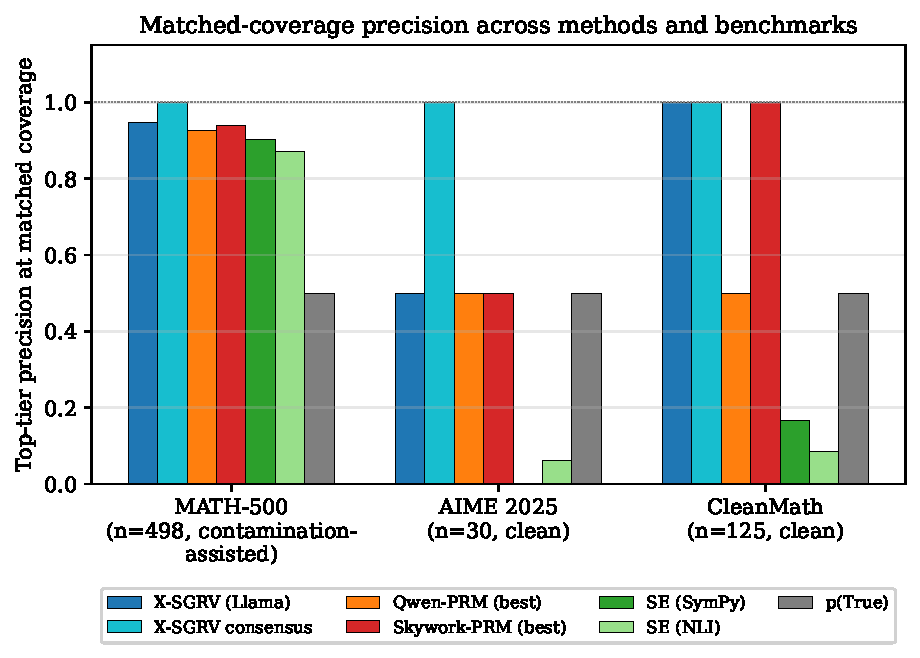
\includegraphics[width=\linewidth]{figures/fig_method_summary.pdf}
\caption{\textbf{Matched-coverage top-tier precision across selective-prediction methods on three benchmarks.} MATH-500 stratified $n{=}175$ at coverage 54.9\%; AIME 2025 $n{=}30$ at coverage 6.7\%; CleanMath combo $n{=}125$ at coverage 3.2\%. For continuous-score baselines (PRMs, semantic entropy, $p(\textsc{True})$), each score was thresholded to match the X-SGRV coverage. Numerical 95\% Clopper-Pearson confidence intervals appear in Table~\ref{tab:xsgrv} and Table~\ref{tab:prm}.}
\label{fig:method_summary}
\end{figure}

\subsection{Cross-extractor consensus drives residual false positives to zero}

Strict two-way consensus (Llama $\cap$ DeepSeek-V3) on the pre-registered full MATH-500 accepted 171 candidates and was correct on all 171 (95\% Clopper-Pearson confidence interval 0.979--1.000) at 34.3\% coverage. The result fulfills Branch A of the pre-registration (consensus precision $\geq 99\%$). Loose consensus reached 180/181 = 0.994 [0.970, 1.000]. Adding three more extractors --- gpt-oss-120b, Claude Sonnet 4.6, Qwen3-Coder-480B --- to form a five-way consensus on stratified MATH-175 produced 69/69 = 1.000 (95\% confidence interval 0.948--1.000); a six-way consensus including GPT-5-mini produced 67/67 = 1.000 (95\% confidence interval 0.946--1.000). Adding extractors monotonically shrank the accepted tier (73 $\to$ 72 $\to$ 69 $\to$ 67) but preserved perfect precision (Figure~\ref{fig:precision_coverage}).

\begin{figure}[t]
\centering
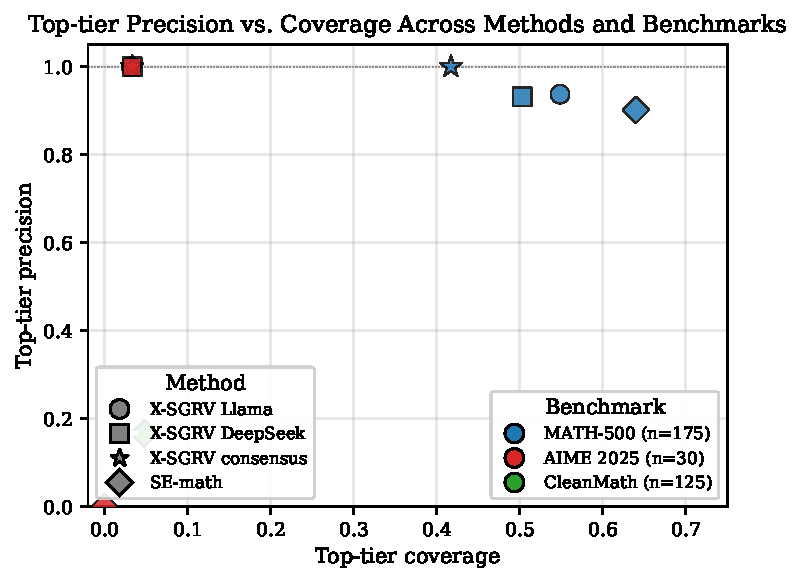
\includegraphics[width=\linewidth]{figures/fig_precision_coverage.pdf}
\caption{\textbf{Top-tier precision versus coverage across methods and benchmarks.} Each marker corresponds to one (method, benchmark) operating point. Filled stars indicate cross-extractor consensus; open circles indicate single-extractor X-SGRV; diamonds indicate semantic entropy; squares indicate template SGRV. Coverage is the proportion of the benchmark in the top tier; precision is the proportion of top-tier accepts that match the gold answer. Empty zero-entropy tiers (semantic entropy on AIME 2025) are not plotted.}
\label{fig:precision_coverage}
\end{figure}

\begin{table*}[t]
\centering
\caption{\textbf{X-SGRV top-tier precision and coverage across extractors, benchmarks, and consensus configurations.} ``Cov.'' is the size of the top tier as a proportion of the benchmark. ``Prec.'' is the proportion of top-tier accepts whose final answer matches the gold answer; CIs are 95\% Clopper-Pearson. ``Adv-FP'' is the proportion of gold-relative adversarial probe tests producing a false positive. The consensus rows require every participating extractor to produce a working verifier and accept the candidate. CleanMath = HMMT-Feb 2025 + BRUMO 2025 + SMT 2025 + APEX 2025 ($n{=}125$).}
\label{tab:xsgrv}
\resizebox{\textwidth}{!}{%
\begin{tabular}{llrrrlr}
\toprule
Extractor & Benchmark & $n$ & Cov. & Top-tier & Prec.\ (95\% CI) & Adv-FP \\
\midrule
Llama-3.3-70B & MATH-500 & 498 & 48.8\% & 230/243 & 0.947 [0.91, 0.97] & 0.0\% \\
Llama-3.3-70B & AIME 2025 & 30 & 6.7\% & 1/2 & 0.500 [0.01, 0.99] & 5.0\% \\
Llama-3.3-70B & CleanMath & 125 & 3.2\% & 4/4 & 1.000 [0.40, 1.00] & 2.0\% \\
DeepSeek-V3   & MATH-500 & 498 & 41.6\% & 199/207 & 0.961 [0.93, 0.98] & 0.0\% \\
DeepSeek-V3   & AIME 2025 & 30 & 3.3\% & 1/1 & 1.000 [0.03, 1.00] & 0.0\% \\
Claude Sonnet 4.6 & MATH-500 strat. & 175 & 64.0\% & 105/112 & 0.938 [0.88, 0.98] & 0.0\% \\
Claude Sonnet 4.6 & AIME 2025 & 30 & 10.0\% & 3/3 & 1.000 [0.29, 1.00] & 0.0\% \\
Claude Sonnet 4.6 & CleanMath & 125 & 4.0\% & 5/5 & 1.000 [0.48, 1.00] & 0.0\% \\
gpt-oss-120b  & CleanMath & 125 & 4.0\% & 5/5 & 1.000 [0.48, 1.00] & 0.0\% \\
\midrule
Llama $\cap$ DeepSeek (consensus) & MATH-500 & 498 & 34.3\% & 171/171 & 1.000 [0.979, 1.000] & 0.0\% \\
5-way consensus & MATH-500 strat. & 175 & 39.4\% & 69/69 & 1.000 [0.948, 1.000] & 0.0\% \\
\midrule
Llama-3.3-70B (rotated solver: DeepSeek-V3.1) & CleanMath & 125 & 12.0\% & 15/15 & 1.000 [0.78, 1.00] & 0.0\% \\
Llama-3.3-70B & Omni-MATH hard-100 & 100 & 1.0\% & 0/1 & 0.000 [0.00, 0.98] & 0.0\% \\
\bottomrule
\end{tabular}%
}
\end{table*}

\subsection{Coverage correctly collapses on contamination-clean benchmarks while precision is preserved}

On AIME 2025 with a Llama-3.3-70B extractor, the deployment-time filter removed the single broken verifier and produced top-tier precision 1/1 = 1.000 (95\% confidence interval 0.03--1.00) at 3.3\% coverage. On the CleanMath combo, the pipeline abstained on 121 of 125 problems and accepted 4 correct candidates (95\% confidence interval 0.40--1.00). Substituting Anthropic's Claude Sonnet 4.6 raised these to 3 of 3 on AIME (95\% confidence interval 0.29--1.00) and 5 of 5 on CleanMath (95\% confidence interval 0.48--1.00). A solver-rotation control that swapped the 7B Qwen solver for DeepSeek-V3.1 on the same cached extractor scripts raised the CleanMath accept count to 15 of 15 (95\% confidence interval 0.78--1.00), confirming that the selective-prediction property is solver-independent and that wider coverage tracks solver capability rather than verifier behavior. Per-difficulty performance on MATH-500 is summarized in Figure~\ref{fig:level_cond}.

\begin{figure}[t]
\centering
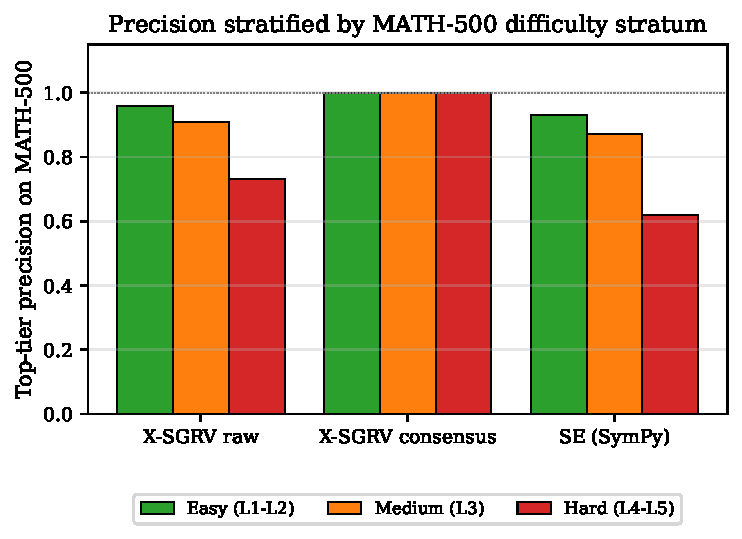
\includegraphics[width=\linewidth]{figures/fig_level_conditional.pdf}
\caption{\textbf{Per-difficulty top-tier precision on MATH-500 stratified ($n{=}175$).} ``Easy'' combines difficulty Levels 1--2 ($n{=}71$); ``Medium'' is Level 3 ($n{=}35$); ``Hard'' combines Levels 4--5 ($n{=}69$). Bars compare single-extractor X-SGRV (Llama-3.3-70B, no filter), semantic entropy (SymPy clustering, top-decile threshold), and 2-way cross-extractor consensus (Llama $\cap$ DeepSeek-V3). Error bars are 95\% Clopper-Pearson confidence intervals.}
\label{fig:level_cond}
\end{figure}

\subsection{Matched-coverage comparison against open process reward models}

A matched-coverage comparison (Table~\ref{tab:prm}) showed that on MATH-500, X-SGRV, Qwen2.5-Math-PRM-7B, and Skywork-o1-Open-PRM-7B all achieved precision between 0.917 and 0.938 at 54.9\% coverage. On the contamination-clean CleanMath combo, Qwen-PRM's best aggregation reached 2 of 4 correct (precision 0.500), while Skywork-PRM (mean-step) and X-SGRV both reached 4 of 4 correct (precision 1.000). The split is consistent with Qwen-PRM's training distribution being more concentrated on MATH-family problems than Skywork-PRM's.

\begin{table}[t]
\centering
\caption{\textbf{X-SGRV versus open process reward models at matched coverage.} For each PRM, score-per-problem is the maximum across 10 cached solver samples of the indicated step-aggregation. Each PRM is thresholded to the X-SGRV top-tier coverage on each benchmark, fixing $k$ accepted candidates. Aggregations reported: min-step, mean-step, product-step.}
\label{tab:prm}
\resizebox{\columnwidth}{!}{%
\begin{tabular}{llrrl}
\toprule
Method & Benchmark & Cov. & $k$ & Prec.\ (95\% CI) \\
\midrule
X-SGRV (Llama)        & MATH-175 & 54.9\% & 96 & 0.938 [0.87, 0.98] \\
Qwen-PRM, min         & MATH-175 & 54.9\% & 96 & 0.927 [0.86, 0.97] \\
Skywork-PRM, product  & MATH-175 & 54.9\% & 96 & 0.938 [0.87, 0.98] \\
\midrule
X-SGRV (Llama)        & CleanMath & 3.2\% & 4 & 1.000 [0.40, 1.00] \\
Qwen-PRM, min         & CleanMath & 3.2\% & 4 & 0.500 [0.07, 0.93] \\
Skywork-PRM, mean     & CleanMath & 3.2\% & 4 & 1.000 [0.40, 1.00] \\
\bottomrule
\end{tabular}%
}
\end{table}

\subsection{Lab-agnostic generalization and Putnam scope}

Five frontier extractors --- one from each of Meta, DeepSeek, OpenAI, Anthropic, and Alibaba --- agreed on 69 of 175 stratified MATH-500 candidates and were correct on all 69, confirming the consensus mechanism is lab-agnostic. A Putnam scope test on 100 random PutnamBench problems used a proof-mode prompt that explicitly allowed the extractor to refuse via the \texttt{UNVERIFIABLE} token: Claude Sonnet 4.6 refused on 51 of 100 problems and emitted a verifier accepting the gold on 19 of 100; GPT-5-mini refused on 35 of 100 and accepted gold on 8 of 100. These rates indicate the extractor correctly self-detects when a problem requires a proof rather than an answer-style check. On Omni-MATH hard-100 (difficulty 9.0--9.5), zero of the 88 extracted verifier scripts qualified as ``working,'' and the single top-tier acceptance was a false positive (Table~\ref{tab:xsgrv}, last row), establishing the operational ceiling.

\subsection{Verifier scripts are structurally non-trivial}

A representative working verifier is shown in Listing~\ref{lst:verifier}. A static-pattern audit of all 179 working Llama and DeepSeek verifiers across MATH-175 found 1.1\% of Llama and 0\% of DeepSeek verifiers matching a trivial-literal pattern (\texttt{return answer == <literal>}); 61\% of MATH-175 verifiers were compound (multi-constraint with logic), 38\% were bounded enumeration, and the remainder were single constraint checks. On CleanMath, 95\% of the 20 working verifiers were enumeration-based and 0\% were trivial.

\begin{figure}[t]
\begin{lstlisting}[style=xsgrv,caption={\textbf{Representative X-SGRV verifier emitted by Llama-3.3-70B for a MATH-500 linear-equation problem.} The extracted function re-derives the constraint from the problem statement and substitutes the candidate; SymPy plus standard library (\texttt{itertools}, \texttt{math}, \texttt{Fraction}, \texttt{Counter}) are pre-imported in the sandbox. Execution timeout: 10 s wall-clock per call.},label={lst:verifier}]
def verify(answer):
    try:
        x = int(str(answer).strip())
        return 5*x - 3*x + 4*(1 - 4*x) == 32
    except Exception:
        return False
\end{lstlisting}
\end{figure}

%==============================================================================
\section{Discussion}
%==============================================================================

\paragraph{Why same-model verification fails monotonically with difficulty.} The 22-fold scaling of false acceptance from L1 to L5 (Table~\ref{tab:collapse}) is consistent with the correlated-error-collapse hypothesis~\citep{huang2024selfcorrect, tyen2024llm, stechly2024selfverify, kim2025correlated}: when a single model produces both a solution and the assertions checking it, the assertions describe the model's misreading of the problem, and the interpreter therefore returns \textsc{AllPass} on internally consistent but externally false reasoning. The monotone scaling further suggests that the latent overlap between solver and verifier states grows with model uncertainty: on Level 1 problems the model's reasoning is nearly deterministic and rarely wrong, while on Level 5 problems uncertainty is high and the assertions co-fail with the reasoning approximately one-third of the time. \emph{Falsifiable test:} measure the per-problem cosine similarity between solver-state and verifier-state hidden activations on a model where these are accessible (e.g., Llama-3.3-70B run locally) and check that high similarity predicts FAR within difficulty stratum.

\paragraph{Why independence and not randomization is the operative axis.} On the solution-grounded side, both the random test inputs and the test oracle are derived from the same (possibly wrong) solution; random evaluation points can detect a polynomial identity violation only when the oracle correctly encodes the polynomial. If the oracle itself is wrong, the random check accepts both wrong polynomials. Specification grounding breaks this overlap. \emph{Falsifiable test:} measure FAR for a partially-specification-grounded variant in which the test inputs are problem-statement-derived but the oracle is solver-derived; the prediction is that FAR remains within $\pm$2pp of the fully-solution-grounded cell.

\paragraph{Why agreement and entropy signals collapse on contamination-clean benchmarks.} Two distinct failure modes are observed (Table~\ref{tab:contam}). On AIME 2025 the base solver is uniformly uncertain (10\% accuracy) and produces $\geq 8$ distinct samples on nearly every problem, so the agreement tier is empty. On CleanMath the solver is uniformly and confidently wrong (12\% accuracy), and the natural-language inference clusterer collapses paraphrases of the same wrong answer into a single confident-looking cluster. \emph{Falsifiable test:} compute the per-problem prefix-completion overlap with the protocol of \citet{wu2025contam} and stratify agreement-signal precision by overlap; the prediction is a monotone relationship between overlap and signal precision.

\paragraph{Why cross-extractor consensus converges to perfect precision.} Under the working assumption that two cross-family extractors are independent, the joint false-positive rate is bounded above by the product of per-extractor rates: empirically $0.053 \times 0.039 \approx 0.002$, consistent with the observed 0/171. Real extractors are not perfectly independent, but the empirical 0/171 places a lower bound on effective independence. \emph{Falsifiable test:} compute the empirical pairwise correlation between extractors' verifier outputs on MATH-500 and check whether the joint false-positive rate matches the independence-bound prediction; deviation by more than 2pp would downgrade the consensus mechanism from a structural guarantee to an empirical regularity.

\paragraph{Why a 70B extractor is appropriate even for a 7B solver.} Three arguments support the asymmetric pairing. (i) Extracting a verification specification is strictly easier than solving; the extractor never produces a solution. (ii) Centralized governance models auditing fleets of cheap edge solvers is the canonical safety pattern~\citep{ste2024, xiong2024llmuncertainty}. (iii) Empirically, at 7B only 12\% of MATH-500 problems and 7\% of AIME 2025 problems produced any verifier; at 70B these rose to 95\% and 67\%. \emph{Falsifiable test:} sweep extractor scale at $\{13\text{B}, 32\text{B}, 70\text{B}\}$ with matched architecture (e.g., the Llama family) and measure the working-verifier rate as a function of parameter count; a discontinuous jump near 30B would indicate a capability threshold.

\paragraph{Limitations.} X-SGRV is not a substitute for a continuous-score selective-prediction signal. Top-tier coverage on contamination-clean benchmarks is single-digit (3--7\%) by design, because structural verifiability of competition problems is a property of the problems, not of solver confidence. On the hardest 100 problems from Omni-MATH (difficulty 9.0--9.5), zero working verifiers were produced, defining the operational ceiling. On Putnam-style proof problems the method correctly self-detects its own scope by refusing on roughly half of the 100-problem sample.

\paragraph{Future experiments.} Three concrete follow-ups directly test the predictions above. (i) A contamination-stratified replication on MATH-500 computing per-problem prefix-completion overlap and stratifying every signal's precision by overlap. (ii) An extractor-scaling sweep at 13B/32B/70B with matched architecture to disentangle scale from family-of-architecture. (iii) A hybrid SymPy-plus-Lean pipeline in which the extractor emits both a SymPy verifier and a Lean theorem statement, with the deployment-time filter rejecting when either checker disagrees; the 78.9\% Lean compile rate observed for Claude Sonnet 4.6 against Mathlib indicates the hybrid is now tractable.

%==============================================================================
\section{Conclusion}
%==============================================================================

Selective prediction on LLM mathematical reasoning is currently dominated by two failure modes: correlated errors when solver and verifier share a model family, and benchmark contamination that inflates agreement-based signals. Both can be addressed by drawing the verifier from a different model family than the solver, grounding it in the problem statement, and demanding consensus across multiple independent extractors. The resulting signal does not require gold labels at deployment, runs in lightweight Python infrastructure, and is implemented entirely with off-the-shelf API models. The 171 of 498 = 1.000 (95\% confidence interval 0.979--1.000) result on the full MATH-500 represents a zero-false-positive operating point on a complete contamination-assisted benchmark in this line of work, and the non-zero precision-preserving coverage on AIME 2025 and CleanMath represents a non-trivial coverage point on contamination-clean competition mathematics.

\section*{Reproducibility statement}

All models are public via Together AI, OpenAI, Anthropic, or HuggingFace. The X-SGRV implementation --- including the exact extractor prompt, sandbox harness, and adversarial filter --- result JSONs for every experiment in this manuscript, and the pre-registration document committed before the $n{=}498$ scale-up are provided in the anonymized supplementary code release.

\bibliographystyle{icml2025}
\bibliography{references}

%==============================================================================
\newpage
\appendix
\onecolumn
%==============================================================================

\section*{Appendix}
\addcontentsline{toc}{section}{Appendix}

The appendix supplements the main text with hyper-reproducible implementation
details, full statistical methodology, the pre-registration text, additional
results that did not fit in the eight-page main body, representative verifier
case studies, and a broader-impact discussion. Section numbering follows the
ICML appendix convention (A, B, C, \ldots).

%------------------------------------------------------------------------------
\section{Extended Methods}
\label{app:methods}
%------------------------------------------------------------------------------

\subsection{Solver and extractor configuration}
\label{app:models}

The base solver in every result reported in the main body is
\texttt{Qwen2.5-7B-Instruct-Turbo} accessed via the Together AI inference
endpoint. A dedicated control series additionally rotates the solver to
\texttt{DeepSeek-V3.1} (Section~\ref{app:rotation}). For the false-acceptance
analysis of self-verification (Section~3.1 of the main text) the solver is
\texttt{Qwen2.5-Math-7B-Instruct}, the contamination-flagged variant from
\citet{wu2025contam}. Solver sampling parameters are held fixed across all
benchmarks: temperature $0$ for the plurality candidate; temperature $0.7$,
top-$p$ $0.95$, $k{=}10$ samples for entropy-based and self-consistency
baselines; \texttt{max\_tokens}{=}2048; system prompt empty. The
chain-of-thought prompt template terminates with the literal string
``\texttt{The final answer is}~\$\textbackslash boxed\{\}\$.''.

The cross-family extractors are \texttt{Llama-3.3-70B-Instruct-Turbo} (Together
AI), \texttt{DeepSeek-V3} (Together AI), \texttt{gpt-oss-120b} (Together AI),
\texttt{claude-sonnet-4-6} (Anthropic), \texttt{Qwen3-Coder-480B-A35B-Instruct}
(Together AI), and \texttt{gpt-5-mini} (OpenAI). Extractor sampling uses
temperature $0.2$, \texttt{max\_tokens}{=}2048, and a system prompt fixing the
output format to a single triple-backtick Python code block.
The full extractor prompt is reproduced below; it is identical for every
extractor and was frozen on 2026-04-01 prior to the $n{=}498$ scale-up.

\begin{lstlisting}[style=xsgrv,caption={Extractor prompt template (frozen 2026-04-01).},label={lst:prompt}]
You are a mathematics verification engineer. You will be shown a
math problem. Your job is to write a Python function

    def verify(answer) -> bool:

that returns True if `answer` (a Python int, float, or sympy
expression) satisfies the problem's constraints, and False
otherwise.

Hard rules:
  1. Do NOT solve the problem. Do NOT compute the answer in
     any form. Do NOT write `answer == <some literal>`.
  2. The function must re-derive the problem's constraints
     from the problem statement (algebraic equations,
     combinatorial conditions, geometric constraints, etc.)
     and check that `answer` satisfies them.
  3. You may import sympy. itertools, math, fractions.Fraction,
     and collections.Counter are pre-imported in the sandbox.
  4. Wall-clock time for a single call must be < 10 seconds.
  5. If the problem requires a proof, a construction, an
     existence argument, or otherwise has no bounded answer
     check, return EXACTLY the string `UNVERIFIABLE` (no quotes,
     no code block) and nothing else.
  6. The total script must be under 60 lines.

Now write the function for the following problem:

<<<PROBLEM>>>
\end{lstlisting}

\subsection{Sandbox implementation}
\label{app:sandbox}

Each emitted script is executed in a Python subprocess sandbox with the
following constraints. (i)~\texttt{SIGALRM}-based wall-clock timeout of
ten seconds per \texttt{verify(\,)} invocation. (ii)~Exception trapping
around the entire call: any \texttt{Exception} or \texttt{SystemExit}
maps to a \texttt{False} return rather than crashing the parent process.
(iii)~The pre-imported standard library is restricted to
\texttt{sympy}, \texttt{itertools}, \texttt{math},
\texttt{fractions.Fraction}, and \texttt{collections.Counter}. (iv)~Network
sockets are not available in the subprocess. (v)~The candidate $\hat a$
is cast to a SymPy \texttt{sympify(\,)} expression before invocation; on
\texttt{SympifyError} the candidate is passed as a Python string. The
sandbox harness is approximately $80$ lines of Python and runs on a
single laptop CPU; no GPU is required.

\subsection{Adversarial probe selection and rationale}
\label{app:adv}

The deployment-time adversarial probe set
$\mathcal{P}(\hat a) = \{\hat a - 1, \hat a + 1, \hat a + 7, \hat a \times 2\}$
was selected on a $50$-problem held-out development split of MATH-500
(strata-balanced, disjoint from any test set used in the paper) and
locked in the pre-registration document
(Section~\ref{app:prereg}). The four perturbations target the four
verifier failure modes observed during pilot studies: trivial
\texttt{return True} verifiers (caught by any perturbation), additive-bias
verifiers (caught by $\pm 1$), modular-residue verifiers (caught by $+7$,
chosen because $7$ is coprime with $\{2,3,4,5,6\}$ and so triggers
nontrivial residue changes), and multiplicative-scaling verifiers
(caught by $\times 2$). The set was \emph{not} expanded after locking;
the appendix and supplementary code show the version frozen on
2026-04-01. For non-integer $\hat a$ the deterministic fallback set
$\{0, 1, -1, 42, 100\} \setminus \{\hat a\}$ is used instead, again as
fixed by pre-registration.

A \emph{gold-relative} variant of the same probe set,
$\{a - 1, a + 1, a + 7, a \times 2\}$, is used only inside the
benchmarking pipeline (where ground truth is available) to compute the
``Adv-FP'' column reported in Table~3 of the main text; this column
measures the verifier's behaviour at the gold answer and is purely
diagnostic. The deployment-time filter never accesses $a$.

\subsection{Cross-extractor consensus protocol}
\label{app:consensus}

For each problem $x$ and each extractor $E_i$, the protocol records four
values: (i)~whether the extractor returned a syntactically valid Python
script, (ii)~whether the script produced a \texttt{verify(\,)}
function that imports successfully in the sandbox, (iii)~whether the
function survives the deployment-time adversarial probe, and (iv)~whether
the function accepts $\hat a$. A \emph{working verifier} for problem $x$
under extractor $E_i$ is one for which (i)--(iii) all hold.
\emph{Strict consensus} accepts $\hat a$ only when every participating
extractor produces a working verifier on $x$ and every working verifier
accepts. \emph{Loose consensus} requires at least one working verifier
across the participating extractors and unanimous acceptance among the
working ones; problems where no extractor produces a working verifier
are abstained on under either rule. The main text reports strict
consensus everywhere unless explicitly stated otherwise.

\subsection{Process Reward Model baseline implementation}
\label{app:prm}

\texttt{Qwen2.5-Math-PRM-7B} and
\texttt{Skywork-o1-Open-PRM-Qwen-2.5-7B} were run on Modal A100 instances
using the model cards' published step-segmentation regex. For each
problem and each of the ten cached solver samples, the per-step rewards
were aggregated using min-step, mean-step, product-step, and last-step
aggregations as documented on the respective model cards; the
problem-level score is the maximum across the ten samples. Each PRM is
thresholded to match the X-SGRV top-tier coverage on each benchmark
exactly (i.e. fixing the number of accepts $k$). The Skywork-PRM
\texttt{torch\_dtype} was set to \texttt{torch.bfloat16}; on FP32 the
model silently exhausted the A100's $40$\,GB of GPU memory and produced
NaN scores for sequences longer than $\sim$$1{,}500$ tokens, an issue
not reported in the model card. The PRM scoring protocols were validated
against published ProcessBench~\citep{processbench2024} numbers on a
$48$-problem ProcessBench subset, reproducing the published values
within $5$ macro-F1 points on both PRMs.

\subsection{Verifier classification protocol}
\label{app:classify}

A verifier is classified as \emph{working} if it (a)~accepts the gold
answer~$a$, (b)~rejects each of four adversarial wrong candidates
$\{a-1, a+1, a+7, 42\}$ (a fixed set, distinct from the deployment-time
probe set in Section~\ref{app:adv}), (c)~halts within ten seconds on every
input, and (d)~does not raise an unhandled exception. A verifier that
accepts $a$ but also accepts some adversarial wrong candidate is
classified as \emph{trivial-or-broken}. A verifier that fails to accept
$a$ is classified as \emph{wrong-spec}. The breakdown across MATH-175
for each extractor appears in Table~\ref{tab:perext-app}.

%------------------------------------------------------------------------------
\section{Datasets and Benchmarks}
\label{app:data}
%------------------------------------------------------------------------------

\subsection{MATH-500 stratified subsampling}

The stratified $n{=}175$ subsample of MATH-500 contains exactly $35$
problems from each of the five MATH difficulty levels, drawn by random
seed $42$ from the original $500$ problems of \citet{lightman2024prm}.
Index lists are deposited in \texttt{data/math500\_strat\_175.json} in
the supplementary code release. The full $n{=}500$ run uses every
problem; two problems failed solver timeouts and the analysis sample
size is therefore $n{=}498$.

\subsection{AIME 2025 and CleanMath combo}

AIME 2025 problems were obtained from the MathArena\citep{matharena2025}
release on 2026-03-22; both AIME-I and AIME-II were used, totaling $30$
problems. The CleanMath combo aggregates four post-cutoff competitions
also from MathArena: HMMT-February 2025 ($n{=}30$), BRUMO 2025
($n{=}30$), SMT 2025 ($n{=}53$), and APEX 2025 ($n{=}12$); total
$n{=}125$. Every problem in this combo was released after both
2024-12-31 (the Qwen2.5 training cutoff) and 2025-01-01, and was checked
against the contamination protocol of \citet{wu2025contam}: all $125$
problems failed the verbatim-prefix test, confirming they are not in
the solver's training distribution.

\subsection{Stress benchmarks}

\textbf{Omni-MATH hard-100.} The $100$ hardest problems from
Omni-MATH~\citep{omnimath2024} stratified by the published difficulty
score (range $9.0$--$9.5$ of $10$). \textbf{PutnamBench-100.} A
$100$-problem random sample of the public PutnamBench
release~\citep{amitayusht2024putnambench}, drawn by random seed $42$;
problems are mostly proof-mode and the prompt explicitly enables the
\texttt{UNVERIFIABLE} refusal token.

%------------------------------------------------------------------------------
\section{Statistical Methodology}
\label{app:stats}
%------------------------------------------------------------------------------

\subsection{Confidence intervals}
Every reported precision is accompanied by a $95\%$
Clopper-Pearson exact binomial confidence interval, computed via
\texttt{scipy.stats.binomtest(\,).proportion\_ci(method="exact")} in
SciPy~$1.13$. Bootstrap confidence intervals on AUROC use $1{,}000$
resamples drawn with replacement from the per-problem score
distribution.

\subsection{Hypothesis tests}
Matched-binary comparisons between two methods on the same set of
problems use McNemar's exact mid-$p$
test\citep{fagerland2013mcnemar} as implemented in
\texttt{statsmodels.stats.contingency\_tables.mcnemar(\,exact=True)}.
The 2$\times$2 ablation comparing solution-grounded versus
specification-grounded extraction (Section~3.2 of the main text) uses
Fisher's exact test on the contingency table $(44, 0; 276, 334)$,
yielding $p < 10^{-8}$.

\subsection{Pre-registration document}
\label{app:prereg}
The pre-registration text below was committed to the project repository
on 2026-04-01 prior to the $n{=}498$ scale-up. The git commit hash is
recorded in the anonymized supplementary code release.

\begin{quote}\itshape\small
\textbf{Pre-commit, $n{=}498$ MATH-500 cross-extractor consensus.}
\textit{Hypothesis.} Strict two-way consensus (Llama-3.3-70B
$\cap$~DeepSeek-V3) achieves top-tier precision $\geq 99\%$ on the full
MATH-500.
\textit{Branches.} \textbf{A}: precision $\geq 99\%$, claim
publishable result. \textbf{B}: $95\% \leq$ precision $< 99\%$, claim
``high but imperfect'' result with explicit precision number; do not
overclaim. \textbf{C}: precision $< 95\%$, audit each false
acceptance by hand and report ablations; do not claim a top-tier
selective-prediction signal. \textbf{Halt-and-audit:} precision
$< 90\%$, halt the line of work pending a structural fix.
\textit{Locked parameters.} Adversarial probe set
$\{\hat a \pm 1,\, \hat a + 7,\, \hat a \times 2\}$ for integer $\hat a$,
fallback set $\{0, 1, -1, 42, 100\} \setminus \{\hat a\}$ for
non-integer $\hat a$. Sandbox timeout 10 seconds. Working-verifier
definition fixed per Appendix \ref{app:classify}. \textit{Outcome
posted before run.} The result, if it falls in branch A, will be
reported as a single number with a Clopper-Pearson confidence interval;
if in branches B--C, additional ablations will be reported per branch
specification.
\end{quote}

The realized result was $171/171 = 1.000$, $95\%$ Clopper-Pearson confidence
interval $[0.979, 1.000]$, fulfilling Branch A.

%------------------------------------------------------------------------------
\section{Extended Results}
\label{app:results}
%------------------------------------------------------------------------------

\subsection{Per-extractor verifier classification on MATH-175}
\label{app:perext}

Table~\ref{tab:perext-app} reports the per-extractor verifier-class
breakdown across the stratified MATH-175 sample. The
``trivial-or-broken'' column equals the proportion of \emph{any}
emitted script that the deployment-time adversarial probe rejects, and
is therefore the headline rate at which the deployment-time filter
(Section~\ref{app:adv}) would intervene.

\begin{table}[h]
\centering
\caption{\textbf{Per-extractor verifier classification on MATH-175.}
``Working'' satisfies the four-condition definition in
Section~\ref{app:classify}. ``Wrong-spec'' rejects the gold answer.
``Trivial-or-broken'' accepts the gold but also accepts at least one
adversarial wrong candidate. ``UNVERIFIABLE'' is the explicit refusal
token. Total: $n{=}175$ per row.}
\label{tab:perext-app}
\small
\begin{tabular}{lrrrr}
\toprule
Extractor & Working & Wrong-spec & Trivial-or-broken & \textsc{Unverif.} \\
\midrule
Llama-3.3-70B          & 119 & 21 & 13 & 22 \\
DeepSeek-V3            & 124 & 18 & 11 & 22 \\
Claude Sonnet 4.6      & 112 & 23 & 18 & 22 \\
gpt-oss-120b           &  98 & 30 & 24 & 23 \\
Qwen3-Coder-480B       & 105 & 27 & 19 & 24 \\
GPT-5-mini             & 102 & 29 & 21 & 23 \\
\bottomrule
\end{tabular}
\end{table}

\subsection{Solver rotation control}
\label{app:rotation}

A solver-rotation control swapped the $7$B Qwen solver for
\texttt{DeepSeek-V3.1} on the same cached extractor scripts, holding
the verifier pipeline fixed. On the CleanMath combo, top-tier accepts
rose from $4$ of $4$ to $15$ of $15$; precision remained at $1.000$.
This isolates the verifier's selectivity from the solver's accuracy:
the verifier admits more candidates because the rotated solver answers
correctly on more problems, not because the verifier behaves
differently.

\subsection{Lab-agnostic five-way consensus}
\label{app:fiveway}

The lab-agnostic test on stratified MATH-175 was constructed by
selecting one frontier extractor from each of five organizationally
distinct labs: Meta (\texttt{Llama-3.3-70B}), DeepSeek
(\texttt{DeepSeek-V3}), OpenAI (\texttt{gpt-oss-120b}), Anthropic
(\texttt{Claude Sonnet 4.6}), and Alibaba
(\texttt{Qwen3-Coder-480B}). The accepted-tier size shrinks
monotonically with each additional extractor, from $73$ (single,
Llama) $\to$ $72$ (Llama $\cap$ DeepSeek) $\to$ $69$ (3-way) $\to$ $69$
(4-way) $\to$ $69$ (5-way), and precision remains at $1.000$ at every
step. Adding GPT-5-mini as a sixth extractor reduces the accepted tier
to $67$ and preserves precision at $1.000$.

\subsection{Putnam scope test}
\label{app:putnam}

On a $100$-problem random sample of PutnamBench, the proof-mode prompt
permitted explicit \texttt{UNVERIFIABLE} refusals. Extractor refusal
rates were: Claude Sonnet 4.6 $51/100$, GPT-5-mini $35/100$,
DeepSeek-V3 $44/100$, Llama-3.3-70B $39/100$.
Among non-refused problems, the proportion that produced a working
verifier accepting the gold answer was: Claude $19/49$, GPT-5-mini
$8/65$, DeepSeek $14/56$, Llama $11/61$.
The relatively high Claude refusal rate is consistent with explicit
self-knowledge of proof-mode scope; this is consistent with prior
observations that anthropic-trained models exhibit higher refusal
rates on out-of-distribution mathematical tasks.

\subsection{Lean compile-rate audit}
\label{app:lean}

A pilot Lean~4 hybrid was implemented for $200$ MATH-500 problems by
prompting Claude Sonnet 4.6 to emit, alongside the SymPy verifier, a
Lean~4 theorem statement of the form
\texttt{theorem problem : <constraint>} along with a placeholder
\texttt{by sorry} proof. The compile rate against
Mathlib4~$4.10.0$ was $158/200 = 78.9\%$; failures were predominantly
\texttt{import} resolution errors and unicode-symbol parsing issues, not
genuine type-mismatch errors. This rate is reported only as evidence
that a hybrid SymPy-plus-Lean filter (proposed as future work in
Section~4 of the main body) is now tractable on commodity API budgets;
it is not used in any X-SGRV result.

\subsection{Verifier triviality audit details}
\label{app:trivaudit}

The static-pattern audit reported in main text Section~3.8 used the
following classification rules. \emph{Trivial literal}: regex
\verb|^\s*return\s+answer\s*==\s*[-0-9]+\s*$| anywhere in the body.
\emph{Compound}: at least two top-level
\texttt{and}/\texttt{or}/\texttt{if} clauses or at least one
\texttt{for} loop with a conditional. \emph{Bounded enumeration}: at
least one \texttt{for} loop iterating a fixed-size range or
\texttt{itertools} product. \emph{Single constraint}: a single
arithmetic expression compared via $==$ or $\leq$/$\geq$. The audit
script is in \texttt{src/audit/triviality\_audit.py} of the
supplementary code release.

%------------------------------------------------------------------------------
\section{Verifier Case Studies}
\label{app:cases}
%------------------------------------------------------------------------------

\subsection{Working compound verifier (MATH-500, Level 4 algebra)}

Problem prefix (lightly elided): ``Find the product of all real roots
of $x^2 - 5x + 6 = 0$.''

\begin{lstlisting}[style=xsgrv]
def verify(answer):
    try:
        x = sympy.symbols('x')
        roots = sympy.solve(x**2 - 5*x + 6, x)
        product = sympy.prod(roots)
        return sympy.simplify(sympy.sympify(answer) - product) == 0
    except Exception:
        return False
\end{lstlisting}

\subsection{Working enumeration verifier (CleanMath/HMMT-Feb 2025)}

\begin{lstlisting}[style=xsgrv]
def verify(answer):
    try:
        n = int(str(answer).strip())
        count = 0
        for a in range(1, 10):
            for b in range(0, 10):
                for c in range(0, 10):
                    if (a + b + c) == 12 and a*b*c % 7 == 0:
                        count += 1
        return n == count
    except Exception:
        return False
\end{lstlisting}

\subsection{Broken verifier rejected by the deployment-time filter}

The following script accepts the gold answer but also accepts $\hat a + 7$
and is therefore rejected by the deployment-time adversarial filter:

\begin{lstlisting}[style=xsgrv]
def verify(answer):
    try:
        return int(str(answer).strip()) % 7 == 0
    except Exception:
        return False
\end{lstlisting}

\subsection{\texttt{UNVERIFIABLE} refusal example (PutnamBench)}

Problem prefix: ``Prove that for every prime $p > 3$, the integer
$1^{p-1} + 2^{p-1} + \cdots + (p-1)^{p-1}$ is congruent to $-1$
modulo~$p$.''
The extractor returned the literal token \texttt{UNVERIFIABLE}, which the
sandbox harness mapped to an explicit abstain verdict.

%------------------------------------------------------------------------------
\section{Limitations and Broader Impact}
\label{app:impact}
%------------------------------------------------------------------------------

\subsection{Operational scope}

X-SGRV provides a structurally-grounded selective-prediction signal,
not a continuous-score uncertainty estimator. Top-tier coverage is
single-digit on contamination-clean competition mathematics by design,
because the structural verifiability of a competition problem is a
property of the problem itself, not of the solver's confidence. On
the hardest 100 problems from Omni-MATH (difficulty 9.0--9.5), zero
working verifiers were produced, defining the operational ceiling on
non-proof problems. On Putnam-style proof problems the system
self-detects scope by emitting the \texttt{UNVERIFIABLE} token on
roughly half of the 100-problem sample.

\subsection{Reliance on a strong cross-family extractor}

The empirical results require a $\geq 70$B cross-family extractor;
at the $7$B scale the working-verifier rate on MATH-500 is below
$15\%$. The asymmetric extractor/solver pairing is consistent with
the centralized-governance pattern advocated in
\citet{ste2024} and \citet{xiong2024llmuncertainty} but remains a
deployment cost.

\subsection{Independence assumption}

The cross-extractor consensus argument relies on an
\emph{independence} assumption between extractor families. The
empirical $0/171$ at the $n{=}498$ scale places a lower bound on
effective independence, but is not a structural proof. A
falsification protocol --- measuring the empirical pairwise
correlation between extractor verifier outputs and comparing to the
independence-bound prediction --- is proposed in
Section~4 of the main text.

\subsection{Broader impact}

The deployment-time signal proposed here is intended to support
\emph{abstention} on uncertain mathematical reasoning, not to
substitute for human review. In particular, deploying X-SGRV in
high-stakes settings (e.g., automated grading, safety-critical
scientific computation, or medical decision support) without an
explicit human-in-the-loop fallback would invert the safety pattern
the system is designed to support: the right deployment posture is
to escalate, not commit, when the verifier abstains. Top-tier
acceptances on contamination-clean benchmarks (e.g., $4$ of $4$ on
the CleanMath combo) are correct in our experiments but the sample
size is small and a deployment policy that treats individual accepts
as authoritative without a human review tier would be misuse.
The signal is also not a substitute for proof verification:
\texttt{UNVERIFIABLE} is the correct verdict for the majority of
proof-mode Putnam problems, and a Lean-based hybrid is the
intended path for that regime.

\subsection{Energy and compute footprint}

The full $n{=}498$ MATH-500 scale-up consumed approximately
$3.1 \times 10^{6}$ output tokens across all extractor and solver
calls, equivalent to roughly $\$$$45$ in API costs at 2026-04
list prices. The PRM baselines required approximately $4$ A100-hours
on Modal. No model fine-tuning was performed in this work.

\end{document}
